\section{Ausblick und zukünftige Entwicklungen}
\subsection{Ausblick YOLO}
Da YOLO ein Open-Source-Modell mit einer aktiven und stetig wachsenden Community ist, wird es kontinuierlich weiterentwickelt und verbessert. Angesichts dieser Dynamik ist davon auszugehen, dass YOLO auch in den kommenden Jahren an Relevanz gewinnen wird. Besonders spannend ist die bereits angekündigte Version YOLOv12, die neue Features und Implementierungen einführen soll mit dem Ziel, die Erkennungsgenauigkeit und Effizienz nochmals deutlich zu steigern.
\subsection{YOLOv12}
Das Schlüsselkonzept von YOLOv12 liegt darin eine neuartige, aufmerksamkeitszentrierte Architektur für die Objekterkennung zu sein, die auf Echtzeitleistung mit hoher Genauigkeit kobiniert.
\subsubsection{Wesentliche Merkmale}
\begin{itemize}
    \item \textbf{Mechanismus der Bereichsaufmerksamkeit:} Effiziente Verarbeitung großer rezeptiver Felder durch Aufteilung der Merkmalskarten in gleich große Regionen, was die Rechenkosten senkt.
    \item \textbf{Resteffiziente Schichtaggregationsnetze (R-ELAN):} Verbesserte Merkmalsaggregation zur Optimierung von Trainingsprozessen bei großen Modellen.
    \item \textbf{Optimierte Aufmerksamkeitsarchitektur:} Minimierung des Speicherzugriffs-Overheads durch FlashAttention, Vermeidung von Positionskodierung und Anpassung der MLP-Verhältnisse.
    \item \textbf{Umfassende Aufgabenunterstützung:} Unterstützung von Objekterkennung, Instanzsegmentierung, Bildklassifizierung, Posenschätzung und orientierter Objekterkennung (OBB).
\end{itemize}
\subsubsection{Unterstütze Aufgaben und Modi}
\begin{figure}[ht]
    \centering
    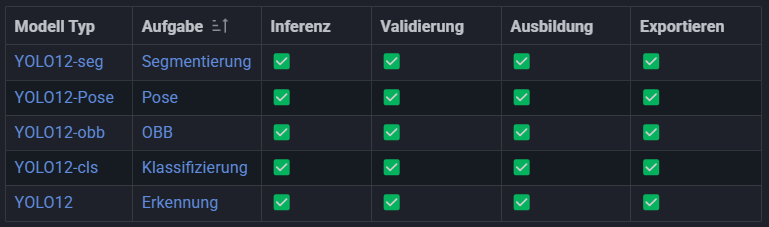
\includegraphics[width=0.85\textwidth]{data/AufgabenUndModiYOLO12.png}
    \caption{Unterstützte Aufgaben und Modis YOLOv12}
    \label{fig:YOLOv12_unterstützte_Modi}
\end{figure}
\subsubsection{Leistungsmetriken}
\textbf{Detektionsleistung (COCO val2017):} YOLO12 zeigt signifikante Verbesserungen in der mAP (mean Average Precision) über alle Modellskalen.\\
\begin{table}[!htbp]
    \centering
    \resizebox{\textwidth}{!}{%
    \begin{tabular}{|l|c|c|c|c|c|l|}
    \hline
    \textbf{Modell} & \textbf{Größe (Pixel)} & \textbf{mAPval 50--95} & \textbf{T4 TensorRT (ms)} & \textbf{Params (M)} & \textbf{FLOPs (B)} & \textbf{Vergleich} \\
    \hline
    YOLO12n & 640 & 40.6 & 1.64 & 2.6 & 6.5 & +2{,}1\% / --9\% (ggü. YOLOv10n) \\
    YOLO12s & 640 & 48.0 & 2.61 & 9.3 & 21.4 & +0{,}1\% / +42\% (ggü. RT-DETRv2) \\
    YOLO12m & 640 & 52.5 & 4.86 & 20.2 & 67.5 & +1{,}0\% / --3\% (vs. YOLO11m) \\
    YOLO12l & 640 & 53.7 & 6.77 & 26.4 & 88.9 & +0{,}4\% / --8\% (ggü. YOLO11l) \\
    YOLO12x & 640 & 55.2 & 11.79 & 59.1 & 199.0 & +0{,}6\% / --4\% (ggü. YOLO11x) \\
    \hline
    \end{tabular}
    }
    \caption{Vergleich verschiedener YOLOv12-Modelle}
    \end{table}

    \subsubsection{Wichtige Verbesserungen}
Das YOLOv12-Modell bringt bedeutende Fortschritte in zwei zentralen Bereichen mit sich. Zum einen wurde die \textbf{Merkmalsextraktion} optimiert, wodurch das Modell große rezeptive Felder effizienter verarbeiten kann. Gleichzeitig wird das Zusammenspiel zwischen aufmerksamkeitbasierten Mechanismen und klassischen Feedforward-Netzwerken gezielter ausbalanciert. Zum anderen überzeugt YOLOv12 durch eine gesteigerte \textbf{architektonische Effizienz}, indem es die Anzahl der Modellparameter reduziert ohne dabei Einbußen bei der Genauigkeit hinzunehmen, teilweise sogar mit Verbesserungen.

\subsubsection{Zusammenfassung und Wichtige Erkenntnisse}
YOLOv12 ist flexibel einsetzbar und deckt viele Bereiche der Computer Vision ab. Dank seiner überarbeiteten Architektur gelingt eine starke Balance zwischen Genauigkeit und Geschwindigkeit. Außerdem unterstützt das Modell verschiedene Modi, was den Einsatz in unterschiedlichsten Anwendungen ermöglicht von Robotik bis hin zur medizinischen Bildverarbeitung.

\subsection{Mikrocomputer gewinnen an Bedeutung}
Mikrocomputer gewinnen in der heutigen Technologie- und Informationsgesellschaft zunehmend an Bedeutung. Ihre kompakte Bauweise, Energieeffizienz und vielseitige Einsetzbarkeit machen sie zu Schlüsselkomponenten in zahlreichen Anwendungen.\\\\
\textbf{Kompakte Bauweise und Energieeffizienz:} Moderne Mikrocomputer sind darauf ausgelegt, hohe Rechenleistung auf kleinem Raum bereitzustellen. Durch fortschrittliche Fertigungstechnologien können sie komplexe Aufgaben effizient bewältigen und dabei den Energieverbrauch minimieren. Dies ist besonders wichtig für mobile Geräte und eingebettete Systeme, bei denen Platz und Energie begrenzt sind.\\\\
\textbf{Vielseitige Einsatzmöglichkeiten:} Die Anwendungsbereiche von Mikrocomputern sind breit gefächert. Sie finden Verwendung in Haushaltsgeräten, Fahrzeugen, medizinischen Geräten, industriellen Steuerungen und vielen weiteren Bereichen. Ihre Fähigkeit, spezifische Aufgaben zuverlässig und effizient zu erfüllen, macht sie in der modernen Technik unverzichtbar.\\\\
\textbf{Unterstützung innovativer Technologien:} Mikrocomputer spielen eine zentrale Rolle bei der Umsetzung neuer Technologien wie de3m Internet of Things (IOT), KI, und der Automatisierung. Sie ermöglichen die Verarbeitung und Analyse von Daten in Echtzeit, was für die Entwicklung intelliegenter Systeme und Anwendungen entscheidend ist.

\subsection{Langlebigkeit des Tutorials}
Durch die Ausarbeitung und erfolgreiche Durchführung des Tutorials mit Studierenden hoffen wir, dass die Technische Hochschule dieses in den kommenden Jahren für die Summer School einsetzen kann. Da das Tutorial bereits in Zusammenarbeit mit Studierenden getestet wurde mit überwiegend positiven Ergebnissen sind wir zuversichtlich hinsichtlich seiner zukünftigen Anwendung. Wie in Abschnitt 7.3 erwähnt, gewinnen Mikrocomputer zunehmend an Bedeutung, was dem Projekt einen zukunftsorientierten Aspekt verleiht. Zudem wird durch die kontinuierliche Weiterentwicklung und Verbesserung des YOLO-Modells auch in den kommenden Jahren eine hohe Relevanz und Anwendungsbedeutung erwartet.

